% ************ Metadata and variables ************ %
\Metadata{
	title=From zero-dimensional theories to inhomogeneous phases with the functional renormalization group,
	author=Martin Jakob Steil,
	subject={},
	keywords={}
}

% ************ Frontmatter ************ %
\frontmatter

\title[From zero-dimensional theories to inhomogeneous phases with the\texorpdfstring{\\}{} functional renormalization group]{From zero-dimensional theories to inhomogeneous phases with the functional renormalization group}
\subtitle[Von null-dimensionalen Theorien zu inhomogenen Phasen mit der\texorpdfstring{\\}{}  funktionalen Renormierungsgruppe]{Von null-dimensionalen Theorien zu inhomogenen Phasen mit der funktionalen Renormierungsgruppe}
\author[Martin Jakob Steil]{M.Sc. Martin Jakob Steil}
\birthplace{Offenbach a. M.}
\submissiondate[\kern1.27em12.12\kern0.01em.202\kern0.01em3]{12.12.2023} % "tell me you have too much time without telling me you have too much time"
\examdate{15.05.2024}
\reviewer{Priv.-Doz. Dr. Michael Buballa \and Prof. Dr. Jens Braun}
\publishers{Darmstadt, Technische Universität Darmstadt}
\department{Fachbereich Physik}
\institute{Institut für Kernphysik Theoriezentrum}
\group{NHQ Group}
\titlegraphic[%
	\phantom{\cite{Koenigstein:2021syz,Koenigstein:2021rxj,Steil:2021cbu,Stoll:2021ori,Koenigstein:2021llr,Steil:2023RGMF,Steil:partIV,Koenigstein:fixedPoint,Koenigstein:2021numericalSchemes}}\\% \phantom{\cite{...}} to ensure 'proper' numbering of references
	\textbf{Cover picture:} Functional renormalization group flow of an instructive toy model in the zero-dimensional $O(N)$ model in the limit $N\rightarrow\infty$. \textit{Adapted from \cref{fig:largeN_0_flow3D}, \ie{}, Fig. 6 of \nbccite{Steil:2021cbu}.}
]{%
	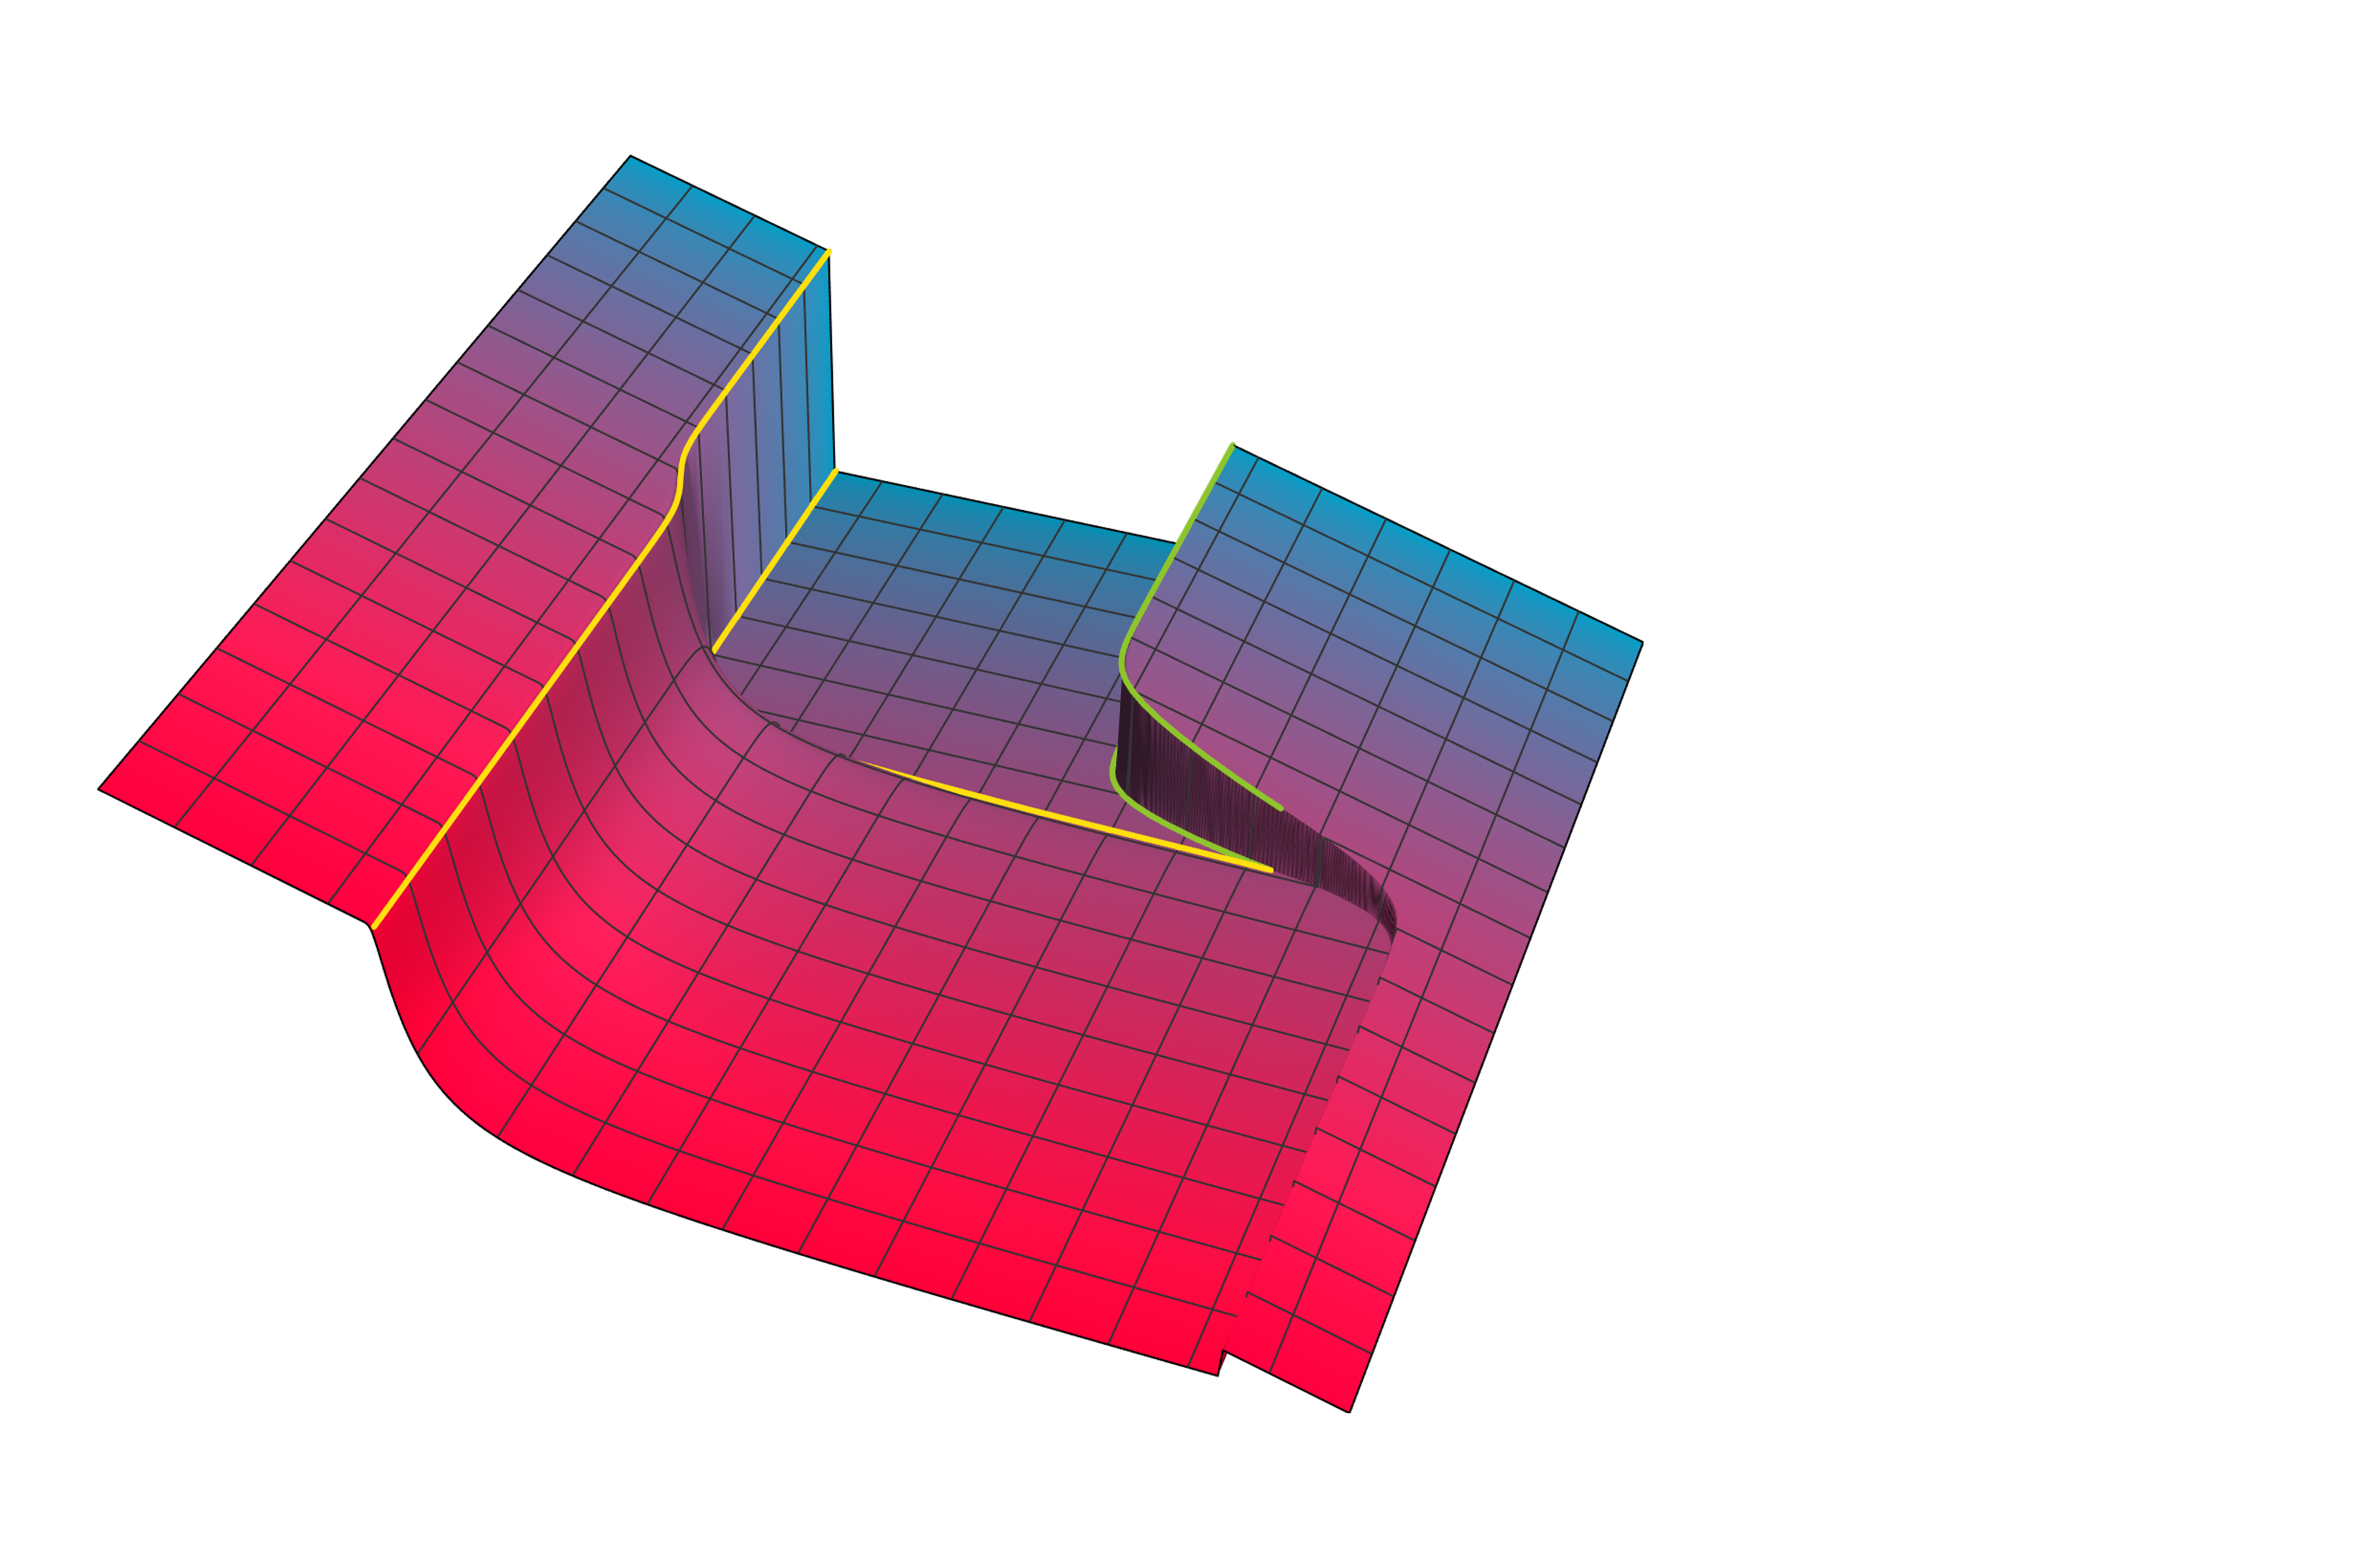
\includegraphics[width=17.9cm]{graphics/titlepage.png}%
}
%\titleaddendum{\textcolor{red}{This revision: \texttt{\commit} on branch \texttt{\branch} compiled on \today\ at \currenttime}}
\sponsors{%
	\begin{minipage}{1.0\textwidth}
		\centering
		\raisebox{-0.5\height}{\href{https://crc-tr211.org/}{\includegraphics[height=1.5cm]{logos/crctr211.eps}}} % 2024.07.31, https://crc-tr211.org/internal/files/logo.zip
		\hspace{4cm}%
		\raisebox{-0.5\height}{\href{https://www.dfg.de/}{\includegraphics[height=1.cm]{logos/dfg.eps}}} % 2024.07.31, https://www.dfg.de/de/service/logo-corporate-design
		\hspace{4cm}%
		\raisebox{-0.5\height}{\href{https://hgs-hire.de/}{\includegraphics[height=1cm]{logos/hgs-hire.eps}}} % 2024.07.31, http://hgs-hire.de/pictures/logo/logo-hgs-hire.eps
	\end{minipage}
}

\tuprints{
	urn=273801,%
	printid=27380,%
	year=2024,
	license=cc-by-sa-4.0,%
	license-logo=\href{https://creativecommons.org/licenses/by-sa/4.0/}{\includegraphics{logos/by-sa.eps}}
}

\dedication{
	\normalsize``McKay (David Hewlett): Yeah, I-I recorded some of my reflections on some of my more ground-breaking accomplishments and theories \ldots uh, just a couple hours worth.\\Teyla (Rachel Luttrell): You should not have gone to so much trouble.''\\
	\small\textit{Stargate Atlantis S4E18 ``The Kindred Part 1'' written by Joseph Mallozzi and Paul Mullie} %[https://stargate.fandom.com/wiki/The_Kindred,_Part_1/Transcript, (accessed on 2021-05-01)]
}

\maketitle % Titlepage, second page, and dedication
\affidavit[signature-location=Rodgau Weiskirchen,signature-image={\includegraphics[width=4cm]{logos/MartinJSteil-Unterschrift}}]

\phantomsection\addcontentsline{toc}{chapter}{Abstract}
\markboth{Abstract}{Abstract}
\begin{abstract}
	% Individual commands to generate standalone abstract
\renewcommand{\ie}{\texorpdfstring{\textit{i.e.}}{i.e.}}
\renewcommand{\viz}{\texorpdfstring{\textit{viz.}}{viz.}}
\renewcommand{\twoDimensional}{\texorpdfstring{${(1 \mkern-3mu + \mkern-3mu 1)}$-dimensional}{(1+1)-dimensional}}
\renewcommand{\fourDimensional}{\texorpdfstring{${(3 \mkern-3mu + \mkern-3mu 1)}$-dimensional}{(3+1)-dimensional}}
\renewcommand{\csb}{\texorpdfstring{$\chi$SB}{χSB}}
%
In this work, we study strongly interacting quantum field theories using the functional renormalization group (FRG) as our primary computational method.
The goal is to facilitate FRG computations in the context of quantum chromodynamics (QCD) to study the phase structure of dense strong-interaction matter.
The main part of this work is split into three chapters, differing in the space-time dimension of the theories under consideration.

We begin by studying zero-dimensional theories, which ultimately involves solving ordinary integrals with complicated FRG flow equations. 
Initially, this might seem like an unnecessarily convoluted way to solve a simple problem.
However, it is this very fact \dash{} applying the FRG to such simple theories \dash{} that allows us to gain enormous insights into the FRG in a rigorous manner.
Arguably, the most relevant development is the novel understanding of FRG flow equations in a fluid-dynamic context.
This allows for the application of methods and concepts from the highly developed field of computational fluid dynamics (CFD) to the FRG.
Two key findings are the identification of bosonic (fermionic) fluctuations as convective (source- or sink-like) contributions to the FRG flow and the resulting link between the CFD concept of numerical entropy and the irreversibility of non-perturbative renormalization group (RG) flows.
These developments serve as a vital stepping stone facilitating the following applications.

We proceed with computations in the \twoDimensional{} Gross-Neveu (GN) model.
We use it to study spontaneous chiral symmetry breaking (\csb{}) \dash{} a phenomenon vital to the understanding of QCD.
Using the previously established CFD methods for the FRG, we study the effects of fermionic and crucially bosonic quantum and thermodynamic fluctuations on spontaneous \csb{}.
The main result of this part of our research is that thermal bosonic fluctuations prevent \csb{} in the \twoDimensional{} GN model.
We further study inhomogeneous \csb{} indirectly using a stability analysis in mean-field (MF) approximation, \ie{}, considering only fermionic fluctuations.
Our research helps to establish this method as a robust tool for both qualitative and quantitative statements about inhomogeneous \csb{}.

We conclude the main part of this thesis with our studies of the \fourDimensional{} Quark-Meson (QM) model, which we primarily consider as a low-energy effective theory of QCD.
We focus on inhomogeneous chiral condensates by studying the QM model within the FRG framework, using a position-dependent ansatz for the chiral condensate, \viz{} the chiral density wave (CDW) for which we have been able to derive explicit FRG flow equations.
We again investigate the effects of fluctuations on spontaneous \csb{} by solving those flow equations in RG-consistent MF calculations.
Thus establishing contact with existing literature results for the QM model with CDW condensates.
These computations \dash{} incorporating only fermionic fluctuations \dash{} are a first step towards a complete solution of the derived flow equations using our established CFD methods.
\end{abstract}

\clearpage
\markboth{Zusammenfassung}{Zusammenfassung}
\begin{abstract}[ngerman]
	% Individual commands to generate standalone abstract
\renewcommand{\twoDimensional}{\texorpdfstring{${(1 \mkern-3mu + \mkern-3mu 1)}$-dimensionalen}{(1+1)-dimensionalen}}
\renewcommand{\fourDimensional}{\texorpdfstring{${(3 \mkern-3mu + \mkern-3mu 1)}$-dimensionalen}{(3+1)-dimensionalen}}
\renewcommand{\csb}{\texorpdfstring{$\chi$SB}{χSB}}
%
In dieser Arbeit untersuchen wir stark wechselwirkende Quantenfeldtheorien unter Verwendung der funktionalen Renormierungsgruppe (FRG) als unsere primäre Rechenmethode.
Das Ziel ist es, FRG-Rechnungen im Kontext der Quantenchromodynamik (QCD) zu ermöglichen, um die Phasenstruktur von dichter, stark wechselwirkender Materie zu studieren.
Der Hauptteil dieser Arbeit ist in drei Kapitel unterteilt, die sich in der Raumzeitdimension der betrachteten Theorien unterscheiden.

Wir beginnen mit dem Studium von null-dimensionalen Theorien, was letztendlich bedeutet, gewöhnliche Integrale mit komplizierten FRG-Flussgleichungen zu lösen.
Dies mag zunächst wie eine unnötig umständliche Methode erscheinen, um ein einfaches Problem zu lösen. 
Es ist jedoch genau diese Tatsache \dash{} die Anwendung der FRG auf solch einfache Theorien \dash{} die es uns auf rigorose Weise ermöglicht, enorme Einblicke in die FRG zu gewinnen.
Die wohl relevanteste Entwicklung ist das neuartige Verständnis der FRG-Flussgleichungen im Kontext der Fluiddynamik.
Dies ermöglicht die Anwendung von Methoden und Konzepten aus dem hochentwickelten Bereich der numerischen Strömungsmechanik (CFD) auf die FRG.
Zwei Schlüsselerkenntnisse sind die Identifizierung von bosonischen (fermionischen) Fluktuationen als konvektive (Quellen- oder Senken-artige) Beiträge zum FRG-Fluss und die daraus resultierende Verknüpfung des CFD-Konzepts der numerischen Entropie und der Irreversibilität von nicht-perturbativen Renormierungsgruppen (RG) Flüssen.
Diese Entwicklungen stellen einen entscheidenden Schritt zur Ermöglichung der folgenden Anwendungen dar.

Wir fahren fort mit Berechnungen im \twoDimensional{} Gross-Neveu (GN) Modell.
Wir verwenden es, um spontane chirale Symmetriebrechung (\csb{}) zu untersuchen \dash{} ein Phänomen, das für das Verständnis von QCD von entscheidender Bedeutung ist.
Mit den zuvor etablierten CFD-Methoden für die FRG untersuchen wir die Auswirkungen von fermionischen und insbesondere bosonischen Quanten- und thermodynamischen Fluktuationen auf spontane \csb{}. 
Das Hauptergebnis dieses Teils unserer Forschung ist, dass thermische bosonische Fluktuationen \csb{} im \twoDimensional{} GN Modell verhindern.
Wir untersuchen des Weiteren inhomogene \csb{} indirekt mittels einer Stabilitätsanalyse in \textit{Mean-Field} (MF) Näherung, d.h. nur unter Berücksichtigung fermionischer Fluktuationen.
Mit unserer Forschung tragen wir dazu bei, diese Methode als robustes Werkzeug für sowohl qualitative als auch quantitative Aussagen über inhomogene \csb{} zu etablieren.

Wir schließen den Hauptteil dieser Arbeit mit unseren Studien zum \fourDimensional{} Quark-Meson (QM) Modell ab, welches wir hauptsächlich als eine effektive Niederenergietheorie von QCD betrachten.
Wir konzentrieren uns auf inhomogene chirale Kondensate, indem wir das QM Modell im Rahmen der FRG untersuchen und dabei einen positionsabhängigen Ansatz für das chirale Kondensat verwenden, namentlich die chirale Dichtewelle (CDW), für die wir explizite FRG-Flussgleichungen ableiten konnten.
Wir untersuchen erneut die Auswirkungen von Fluktuationen auf spontane \csb{}, indem wir diese Flussgleichungen im Rahmen von RG-konsistenten MF Rechnungen lösen.
Dadurch stellen wir eine Verbindung zu bestehenden Literaturergebnissen für das QM Modell mit CDW Kondensaten her.
Diese Berechnungen \dash{} die derzeit nur fermionische Fluktuationen berücksichtigen \dash{} sind ein erster Schritt hin zu einer vollständigen Lösung der abgeleiteten Flussgleichungen unter Verwendung unserer etablierten CFD-Methoden.
\end{abstract}

\clearpage

\phantomsection\addcontentsline{toc}{chapter}{Contents}
{
	\hypersetup{linkcolor=black}
	\microtypesetup{protrusion=false} % disables protrusion locally for toc
	\tableofcontents % prints Table of Contents
}